% !TEX spellcheck = en_US

\documentclass[conference]{IEEEtran}
\usepackage{cite}
\usepackage{amsmath,amssymb,amsfonts}
\usepackage{algorithmic}
\usepackage{graphicx}
\usepackage{textcomp}
\usepackage{xcolor}
% add hyperlinks, delete all .aux files if adding hyperref after previous build
\usepackage{hyperref}
% support for unicode charcters like "é" and "ñ"
\usepackage[T1]{fontenc}
% Provides generic commands \degree, \celsius, \perthousand, \micro and \ohm
\usepackage{gensymb}
% splits a section into multiple columns
\usepackage{multicol}
% balance columns on lastpage
% better than \flushend according to
% https://texfaq.org/FAQ-balance
%\usepackage{flushend}

\def\BibTeX{{\rm B\kern-.05em{\sc i\kern-.025em b}\kern-.08em
    T\kern-.1667em\lower.7ex\hbox{E}\kern-.125emX}}
\begin{document}

\title{Effects of Satellite Sampling on Subhourly Modeling Errors}

\author{\IEEEauthorblockN{Mark A. Mikofski, William F. Holmgren, Jeffrey Newmiller, and Rounak Kharait}
\IEEEauthorblockA{DNV, Oakland, CA, 94612, USA }}

\maketitle

\begin{abstract}
Modeling errors due to hourly inputs averaged from high frequency measurements are significant where solar resource variability and inverter loading ratio are both high. However, solar resource inputs from satellite data are averaged from low frequency measurements. Therefore, we studied the effects of satellite sampling rate on modeling errors by simulating satellite data using high frequency measurements from 8 different locations across the United States. We simulated satellite data by selecting instantaneous measurements at various sampling rates and averaging them to hourly. We observed increasing modeling errors for sampling rates 30-minutes or shorter. For sampling rates longer than 30-minutes, modeling errors decreased, canceling out due to the randomness of the low frequency sampled data. We examined modeling errors further and observed that clipping errors dominated modeling errors from other sources like transposition to POA or DC energy conversion. Based on our observations, we recommend that an hourly modeling correction be applied whenever hourly inputs are used, especially at sites with high solar variability and DC/AC ratios greater than one.
\end{abstract}

\begin{IEEEkeywords}
inverter, clipping, satellite, sampling, solar resource, irradiance, variability, performance, modeling, TMY
\end{IEEEkeywords}

\section{Introduction}
Accurate solar energy assessments are important for lowering the cost of capital for PV systems. However, continuing under-performance of solar assets over the past few years may be damaging investor confidence \cite{Matsui2021}. Several studies have examined potential sources of under-prediction, and modeling errors due to hourly inputs have recently received renewed interest \cite{Parikh2021,Anderson2020,Bradford2020,Kharait2020,Cormode2019}. These modeling errors arise from differences in predicted clipping losses and energy output between using hourly versus subhourly input. When hourly input is time-averaged from high frequency subhourly measurements, energy output is over-predicted and clipping losses are under-predicted. However, satellite data is generated from low frequency measurements that are sampled at 15-minute or 30-minute intervals \cite{Wilcox2012,Sengupta2018}. Recently, a few studies have investigated the difference between hourly input time-averaged from high frequency versus input generated from low frequency sampled data and have demonstrated that modeling errors appear to be reduced for slower sampled data \cite{Bowersox2021}. This study examines the impact of sampling rate on modeling error by simulating satellite data at various frequencies from high frequency ground measurements at the NIST ground array \cite{Boyd2017,Boyd2017a,Boyd2017b} and the 7 SURFRAD stations \cite{Augustine2000}. In the following sections we describe our methods, show our results, and discuss our observations.

\section{Methods}

\subsection{NIST Ground Array Configuration}
For the first part of this study, we used the NIST ground array, a fixed-tilt 260-kW PV system \cite{Boyd2017,Boyd2017a,Boyd2017b}, as the base system and varied the inverter loading ratio by adding additional DC capacity with the same pitch and racking as the existing rows. A weather station at the site collects inputs at 1-minute frequency, allowing simulation of satellite data at any sampling rate. We used SolarFarmer \cite{solarfarmer2018} to simulate a fictitious version of the NIST ground array with a DC/AC ratio of 1.5, because SolarFarmer can use inputs at any frequency.

\subsection{Generic Array Configuration for SURFRAD}
For the second part of this study, we used an imaginary system consisting of a strings of generic 300-W mono-crystalline silicon modules (Canadian Solar CS6X-300M) connected to a single generic 250kW central inverter (SMA America SC250U (480V)), such that the DC/AC ratio was 1.3. The module and inverter parameters were sourced from the NREL System Advisor Model (SAM) libraries \cite{Freeman2018}. High frequency 1-minute input from SURFRAD \cite{Augustine2000} was used with pvlib python \cite{pvlib2018} to predict plane of array (POA) irradiance components, effective irradiance, cell temperature, DC power, and AC output. The method was based on a previous study \cite{9519024} with minor differences. SURFRAD data was filtered for data quality and only years containing at least 98\% complete set of global horizontal irradiance (GHI), diffuse horizontal irradiance (DHI), direct normal irradiance (DNI), air temperature, wind speed, relative humidity, pressure, and solar zenith were used. The SURFRAD irradiance components were checked for self consistency 

\begin{equation}
GHI = 
\end{equation}


\subsection{Input Data}
This study uses a method similar to others to simulate low-frequent satellite data from higher frequency measurements \cite{Bowersox2021}. Although this method can't exactly simulate the complex algorithms used to generate satellite data, we believe it is sufficient to study modeling errors caused by using low frequency inputs. Using only the month of July, 2017, we created 15 difference sets of irradiance input from the 1-minute onsite ground station measurements to study the effect of sampling rate and time averaging on the modeling error. The various datasets can be grouped broadly into three categories: "time-averaged", "instantaneous", "simulated satellite" each with 5 datasets that have either time-averaged or instantaneously sampled data at the following intervals or frequencies:

\begin{itemize}
    \item 1-minute
    \item 5-minutes
    \item 15-minutes
    \item 30-minutes
    \item 60-minutes
\end{itemize}

\emph{Time-averaged}: The first 5 datasets were time-averaged at the different intervals to replicate the modeling error observed when high frequency input data is aggregated. \emph{Instantaneous}: The second 5 datasets were generated by selecting an instantaneous 1-minute record from the onsite measurements. For example, to generate the 15-minute sampled data, only 4 records were selected at the 7th, 22nd, 37th, and 52nd minutes as shown in Fig.~\ref{fig:sampling-diagram}. Note that both the 1-minute "time-averaged" and "instantaneous" datasets are actually identical, because 1-minute was the resolution of the measured data. \emph{Simulated-satellite}: The last 5 datasets simulate satellite data by averaging the records in the "instantaneous" datasets to 1-hour. For example, to generate the 15-minute simulated satellite data, the 4 records shown in Fig.~\ref{fig:sampling-diagram} were averaged together to create one value for that hour. Note that the 60-minute "time-averaged" and 1-minute "simulated satellite" datasets are also identical because they both aggregate the 1-minute measured data to hourly. Also note that all of the "simulated satellite" data contain hourly inputs, while the "time-averaged" and "instantaneous" inputs have the resolutions given by the time-averaging interval or the instantaneous sampling rate.

\begin{figure}[htbp]
\centerline{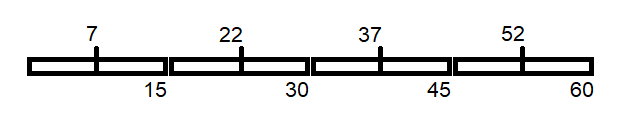
\includegraphics[width=9cm]{sampling-diagram.png}}
\caption{This diagram demonstrates how records were selected to generate 15-minute sampled datasets by selecting only 4 records at the 7th, 22nd, 37th, and 52nd minutes. Then to simulate satellite data, these 4 instantaneous records were averaged together to create a single value for the hour.}
\label{fig:sampling-diagram}
\end{figure}

\section{Results}
\label{section:results}

\subsection{Analysis}
The energy yield and clipping losses for each of the 15 SolarFarmer predictions are shown in Table~\ref{table:results-summary}. A plot of the "time-averaged" inputs is shown in Fig.~\ref{fig:time-averaged}. The 1-minute measurements correctly account for rapid ramp rates in the solar resource when predicting energy yield and clipping loss. However as the time-averaging interval increases, the energy yield is over-predicted and the clipping loss is under-predicted relative to the 1-minute measurements. Blue and orange arrows show the over-predicted energy and under-predicted clipping loss when using hourly "time-averaged" input.

\begin{table}[htbp]
\caption{Summary of SolarFarmer Results}
\begin{center}
\begin{tabular}{|c|c|c|c|}
\hline
\textbf{Dataset} & \textbf{\textit{Interval}}& \textbf{\textit{Energy Yield}}& \textbf{\textit{Clipping Loss}} \\
                 & \textit{minutes}& \textit{kWh/kWp}& \textit{\%} \\
\hline
             &  1& 137.6& -3.4 \\
             &  5& 139.3& -3.1 \\
time-averaged& 15& 140.9& -2.7 \\
             & 30& 141.8& -2.5 \\
             & 60& 142.4& -2.3 \\
\hline
             &  1& 137.6& -3.4 \\
             &  5& 137.8& -3.5 \\
instantaneous& 15& 138.1& -3.5 \\
             & 30& 136.7& -3.5 \\
             & 60& 138.4& -3.4 \\
\hline
             &  1& 142.4& -2.3 \\
simulated-   &  5& 142.1& -2.6 \\
satellite    & 15& 142.0& -2.6 \\
             & 30& 138.8& -3.0 \\
             & 60& 138.4& -3.4 \\
\hline
\end{tabular}
\label{table:results-summary}
\end{center}
\end{table}

The "instantaneous" results are shown in Fig.~\ref{fig:instantaneous}. The 1-minute results are identical to the 1-minute "time-averaged" shown in Fig.~\ref{fig:time-averaged}, because the measurement resolution is every minute. As input data is sampled at lower frequency (longer sampling rates), random errors occur in the input data and cancel out the modeling error.

\begin{figure}[htbp]
\centerline{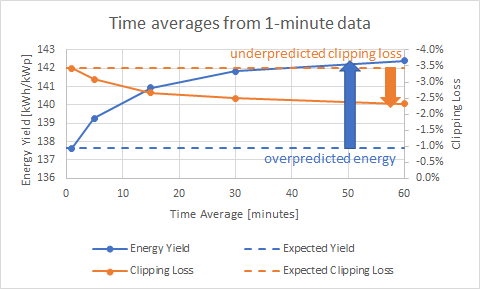
\includegraphics[width=9cm]{time-averaged.png}}
\caption{Energy yield (in blue on left axis) and clipping losses (in orange on right axis) are calculated using "time-averaged" inputs. Dashed lines show the expected output. Blue and orange arrows show the modeling errors when using hourly "time-averaged" input.}
\label{fig:time-averaged}
\end{figure}

\begin{figure}[htbp]
\centerline{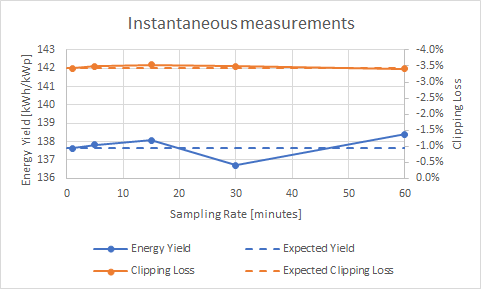
\includegraphics[width=9cm]{instantaneous.png}}
\caption{Energy yield (in blue on left axis) and clipping losses (in orange on right axis) are calculated using "instantaneous" inputs. Dashed lines show the expected output. As input data is sampled less frequently, random errors in the input data cancel out modeling error.}
\label{fig:instantaneous}
\end{figure}

\begin{figure}[htbp]
\centerline{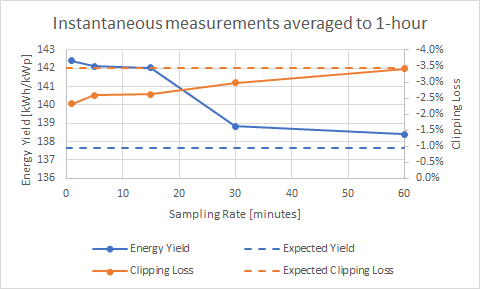
\includegraphics[width=9cm]{satellite-simulated.png}}
\caption{Energy yield (in blue on left axis) and clipping losses (in orange on right axis) are calculated using "simulated-satellite" inputs. Dashed lines show the expected values. As input data is sampled at increasing frequency, the modeling errors become more apparent.}
\label{fig:satellite-simulated}
\end{figure}

The "simulated-satellite" results are shown in Fig.~\ref{fig:satellite-simulated}. The 1-minute results are identical to the 60-minute "time-averaged" shown in Fig.~\ref{fig:time-averaged}, because they both show 1-minute measurements averaged hourly. As input data is sampled at increasing frequency (shorter sampling rates), the modeling errors become more apparent. Because all of the "simulated-satellite" input is hourly, this trend is similar but opposite to the increase in modeling errors observed in "time-averaged" input as the interval is increased. The inflection point seems to be around 30-minutes. At sampling times longer than 30-minutes, random errors occur in the input data and cancel out the modeling error, similar to observations of the "instantaneous" input. However, we observe that even at input data sampled every 30-minutes, which is similar to TMY3, there is still non-zero modeling error.

\subsection{Discussion}
Several studies have already demonstrated the modeling errors observed in Fig.~\ref{fig:time-averaged} due to using hourly averaged input. Newer studies have also shown the apparent reduction in errors due to using "instantaneous" data due to random errors as shown in Fig.~\ref{fig:instantaneous}. This study demonstrates that there are still modeling errors when using satellite data even at 30-minute sampling rates as shown in Fig.~\ref{fig:satellite-simulated}. We also demonstrate that modeling errors will be even larger for satellite data sampled every 15-minutes or faster. From this study we recommend that modeling error corrections be applied whenever hourly input data is used. From this preliminary study, we infer that subhourly modeling errors may be halved when using satellite data, but more study is required. Therefore in the final draft of this paper we propose to repeat this study using full years and solar resource from SURFRAD in addition to the NIST weather station.

\section{Conclusions}
Accurate predictions of energy output are important for decreasing the cost of capital for PV systems, but reports of under-performance for the past few years could damage investor confidence. Many sources of under-predictions have been studied, and subhourly modeling errors have been observed when using hourly input data for sites with high solar variability and DC/AC greater than one. However, satellite data is averaged from coarsely sampled instantaneous measurements with random hourly errors that appear to reduce subhourly modeling errors. This paper examines the effect of sampling rate on subhourly modeling errors by simulating satellite data from high frequency ground measurements at the NIST ground array and predicting energy output at the site using SolarFarmer. We observe modeling errors for simulated satellite input sampled every 30-minutes or shorter, and the errors increase as sampling is more frequent. Therefore, we recommend applying a subhourly modeling error correction whenever hourly input is used. This correction may be halved if using satellite data, but we are working on a more rigorous study. The final draft of this paper will contain results from all of the SURFRAD sites in addition to the NIST data to more accurately quantify the correction factor applied for satellite data.

\bibliographystyle{IEEEtran}
% argument is your BibTeX string definitions and bibliography database(s)
\bibliography{IEEEabrv,bibliography}
%\balance

\end{document}
